% =========================================================================
% BÀI 20: ÔN TẬP CHUNG (TỔNG HỢP TOÀN BỘ HỌC KÌ 1 - TOÁN LỚP 1)
% TOÀN BỘ CÂU HỎI ĐƯỢC VẼ HÌNH MINH HỌA TRỰC QUAN 100% BẰNG TIKZ 2D & 3D
% =========================================================================

% --- CÁC HÀM VẼ HÌNH TRỰC QUAN CHO BÀI 20 ---

\providecommand{\VeKhoiLapPhuong}[4][yellow!60]{% #1=màu, #2=x, #3=y, #4=cạnh
  \begin{scope}[shift={(#2,#3)}]
    \pgfmathsetmacro{\s}{#4}
    \pgfmathsetmacro{\dx}{\s*0.42}
    \pgfmathsetmacro{\dy}{\s*0.32}
    \draw[fill=#1, draw=black!75, line width=1.1pt] (0,0) rectangle (\s,\s);
    \draw[fill=white!35!#1, draw=black!75, line width=1.1pt] (0,\s) -- (\s,\s) -- (\s+\dx,\s+\dy) -- (\dx,\s+\dy) -- cycle;
    \draw[fill=black!25!#1, draw=black!75, line width=1.1pt] (\s,0) -- (\s+\dx,\dy) -- (\s+\dx,\s+\dy) -- (\s,\s) -- cycle;
  \end{scope}
}

\providecommand{\VeKhoiHopChuNhat}[6][cyan!50]{% #1=màu, #2=x, #3=y, #4=rộng, #5=cao, #6=sâu
  \begin{scope}[shift={(#2,#3)}]
    \pgfmathsetmacro{\w}{#4}
    \pgfmathsetmacro{\h}{#5}
    \pgfmathsetmacro{\dx}{#6*0.42}
    \pgfmathsetmacro{\dy}{#6*0.32}
    \draw[fill=#1, draw=black!75, line width=1.1pt] (0,0) rectangle (\w,\h);
    \draw[fill=white!35!#1, draw=black!75, line width=1.1pt] (0,\h) -- (\w,\h) -- (\w+\dx,\h+\dy) -- (\dx,\h+\dy) -- cycle;
    \draw[fill=black!25!#1, draw=black!75, line width=1.1pt] (\w,0) -- (\w+\dx,\dy) -- (\w+\dx,\h+\dy) -- (\w,\h) -- cycle;
  \end{scope}
}

\providecommand{\VeTao}[3][red]{% #1=màu, #2=x, #3=y
  \begin{scope}[shift={(#2,#3)}, scale=0.42]
    \shadedraw[left color=#1!80!black, right color=orange!80!yellow, draw=red!90!black, line width=0.8pt]
      (-0.35,0.1) .. controls (-0.5,0.7) and (-0.1,0.9) .. (0,0.65)
      .. controls (0.1,0.9) and (0.5,0.7) .. (0.35,0.1)
      .. controls (0.3,-0.5) and (-0.3,-0.5) .. (-0.35,0.1);
    \draw[brown!70!black, line width=1.5pt] (0,0.65) .. controls (0.05,0.85) .. (0.15,1.0);
    \fill[green!70!black] (0.08,0.82) .. controls (0.3,0.95) and (0.35,0.75) .. (0.1,0.75) -- cycle;
  \end{scope}
}

\providecommand{\VeGaCon}[3]{% #1=x, #2=y, #3=số
  \begin{scope}[shift={(#1,#2)}, scale=0.8]
    \fill[yellow!90!orange] (0,0) circle (0.38cm);
    \fill[yellow!90!orange] (0.28,0.28) circle (0.25cm);
    \fill[orange] (0.48,0.28) -- (0.68,0.24) -- (0.48,0.18) -- cycle;
    \fill[black] (0.35,0.34) circle (0.04cm);
    \draw[fill=white, draw=black!80, line width=0.8pt, rounded corners=2pt] (-0.3,-0.45) rectangle (0.3,-0.05);
    \node[font=\bfseries\normalsize] at (0,-0.25) {#3};
  \end{scope}
}

% =========================================================================
% PHẦN 1: TRẮC NGHIỆM LỰA CHỌN (12 CÂU) - ĐÁP ÁN ĐƯỢC PHÂN BỔ ĐỀU A, B, C, D
% =========================================================================
\textbf{Phần 1. Trắc nghiệm lựa chọn}
\setcounterpageref{ex}{0}

% --- CÂU 1 ---
\begin{ex} %[1D5N20]
Bác lái tàu đang nối thêm toa số vào đoàn tàu. Số ở toa liền sau của toa mang số $9$ là số nào?
\begin{center}
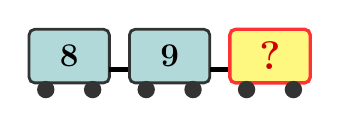
\begin{tikzpicture}[scale=0.85, baseline=(current bounding box.center)]
  % Toa 8
  \draw[fill=teal!30, draw=black!80, rounded corners=2pt, line width=1pt] (0,0) rectangle (1.2,0.8);
  \node[font=\bfseries\large] at (0.6,0.4) {8};
  \fill[black!80] (0.25,-0.1) circle (0.13cm); \fill[black!80] (0.95,-0.1) circle (0.13cm);
  \draw[line width=1.5pt] (1.2,0.2) -- (1.5,0.2);
  % Toa 9
  \draw[fill=teal!30, draw=black!80, rounded corners=2pt, line width=1pt] (1.5,0) rectangle (2.7,0.8);
  \node[font=\bfseries\large] at (2.1,0.4) {9};
  \fill[black!80] (1.75,-0.1) circle (0.13cm); \fill[black!80] (2.45,-0.1) circle (0.13cm);
  \draw[line width=1.5pt] (2.7,0.2) -- (3.0,0.2);
  % Toa ?
  \draw[fill=yellow!50, draw=red!80, line width=1.2pt, rounded corners=2pt] (3.0,0) rectangle (4.2,0.8);
  \node[font=\bfseries\Large, text=red!80!black] at (3.6,0.4) {?};
  \fill[black!80] (3.25,-0.1) circle (0.13cm); \fill[black!80] (3.95,-0.1) circle (0.13cm);
\end{tikzpicture}
\end{center}
\choice
{\True $10$}
{$8$}
{$7$}
{$6$}
\loigiai{
Số liền sau của số $9$ là số $10$.\\
\textbf{Đáp án của câu hỏi là A}
}
\end{ex}

% --- CÂU 2 ---
\begin{ex} %[1D5N20]
Trong giỏ có $5$ quả táo đỏ và $4$ quả táo vàng. Hỏi có tất cả bao nhiêu quả táo?
\begin{center}
\begin{tikzpicture}[scale=0.85, baseline=(current bounding box.center)]
  \draw[fill=orange!20!yellow, draw=brown!80!black, rounded corners=6pt, line width=1.1pt] (-0.3,-0.5) rectangle (7.8,1.7);
  \foreach \i in {0,...,4}{ \VeTao[red]{\i*0.7+0.3}{0.2} }
  \node[font=\bfseries\Large, text=blue!80!black] at (3.8,0.25) {$+$};
  \foreach \i in {0,...,3}{ \VeTao[yellow!90!orange]{\i*0.7+4.5}{0.2} }
  \node[above, font=\bfseries\footnotesize, text=blue!90!black] at (3.75,1.25) {$5 + 4 = ?$ quả};
\end{tikzpicture}
\end{center}
\choice
{$8$}
{\True $9$}
{$10$}
{$7$}
\loigiai{
Phép tính: $5 + 4 = 9$ quả táo.\\
\textbf{Đáp án của câu hỏi là B}
}
\end{ex}

% --- CÂU 3 ---
\begin{ex} %[1D5H20]
Trên cành cây có $10$ chú chim, sau đó $7$ chú chim bay đi tìm mồi. Hỏi trên cành còn lại bao nhiêu chú chim?
\begin{center}
\begin{tikzpicture}[scale=0.85, baseline=(current bounding box.center)]
  \draw[line width=3pt, brown!80!black] (0,0.5) -- (7.8,0.5);
  \foreach \i in {0,...,2}{
    \fill[blue!70!black] (\i*0.8+0.5, 0.7) circle (0.22cm);
  }
  \node[font=\footnotesize\itshape, text=blue!80!black] at (1.3, 0) {Còn lại};
  \foreach \i in {0,...,6}{
    \begin{scope}[shift={(3.2+\i*0.65, 0.7)}]
      \fill[gray!40] (0,0) circle (0.22cm);
      \draw[line width=1.3pt, red] (-0.15,-0.15) -- (0.15,0.15);
      \draw[line width=1.3pt, red] (-0.15,0.15) -- (0.15,-0.15);
    \end{scope}
  }
  \node[font=\footnotesize\itshape, text=red!80!black] at (5.2, 0) {Bay đi ($7$ con)};
\end{tikzpicture}
\end{center}
\choice
{$2$}
{$4$}
{\True $3$}
{$5$}
\loigiai{
Phép tính: $10 - 7 = 3$ (chú chim).\\
\textbf{Đáp án của câu hỏi là C}
}
\end{ex}

% --- CÂU 4 ---
\begin{ex} %[1D5H20]
Quan sát đĩa cân thăng bằng dưới đây. Dấu so sánh thích hợp điền vào dấu hỏi chấm là:
\begin{center}
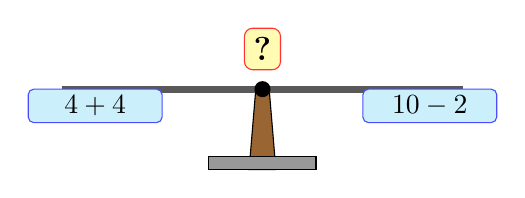
\begin{tikzpicture}[scale=0.85, baseline=(current bounding box.center)]
  % Trục cân
  \draw[fill=brown!80!black] (3.8,-0.7) -- (4.2,-0.7) -- (4.1,0.5) -- (3.9,0.5) -- cycle;
  \draw[fill=gray!80] (3.2,-0.7) rectangle (4.8,-0.5);
  % Đòn cân
  \draw[line width=2.5pt, gray!70!black] (1,0.5) -- (7,0.5);
  \fill[black] (4,0.5) circle (0.12cm);
  % Hai đĩa
  \draw[line width=1pt] (1.5,0.5) -- (1.5,0);
  \draw[fill=cyan!20, draw=blue!70, rounded corners=2pt] (0.5,0) rectangle (2.5,0.5);
  \node[font=\bfseries] at (1.5,0.25) {$4 + 4$};
  
  \draw[line width=1pt] (6.5,0.5) -- (6.5,0);
  \draw[fill=cyan!20, draw=blue!70, rounded corners=2pt] (5.5,0) rectangle (7.5,0.5);
  \node[font=\bfseries] at (6.5,0.25) {$10 - 2$};
  
  \node[draw=red!80, fill=yellow!30, rounded corners=3pt, font=\bfseries\large] at (4,1.1) {?};
\end{tikzpicture}
\end{center}
\choice
{$>$}
{$<$}
{$+$}
{\True $=$}
\loigiai{
Ta có $4 + 4 = 8$ và $10 - 2 = 8$. Vì hai bên đều bằng $8$ nên điền dấu $=$.\\
\textbf{Đáp án của câu hỏi là D}
}
\end{ex}

\newpage

% --- CÂU 5 ---
\begin{ex} %[1D5H20]
Sơ đồ tách gộp số $10$ dưới đây còn thiếu số nào ở dấu hỏi chấm?
\begin{center}
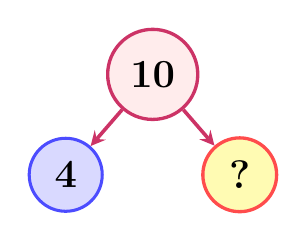
\begin{tikzpicture}[scale=0.85, baseline=(current bounding box.center)]
  \node[circle, draw=purple!80, fill=pink!30, line width=1.2pt, font=\bfseries\Large, inner sep=5pt] (top) at (2,1.5) {10};
  \node[circle, draw=blue!70, fill=blue!15, line width=1.1pt, font=\bfseries\Large, inner sep=5pt] (left) at (0.7,0) {4};
  \node[circle, draw=red!70, fill=yellow!30, line width=1.2pt, font=\bfseries\Large, inner sep=5pt] (right) at (3.3,0) {?};
  \draw[->, >=stealth, line width=1.3pt, purple!80] (top) -- (left);
  \draw[->, >=stealth, line width=1.3pt, purple!80] (top) -- (right);
\end{tikzpicture}
\end{center}
\choice
{$5$}
{\True $6$}
{$7$}
{$8$}
\loigiai{
Số $10$ gồm $4$ và $6$ (vì $4 + 6 = 10$).\\
\textbf{Đáp án của câu hỏi là B}
}
\end{ex}

% --- CÂU 6 ---
\begin{ex} %[1H5H20]
Trong các hình dưới đây, hình nào là hình vuông?
\begin{center}
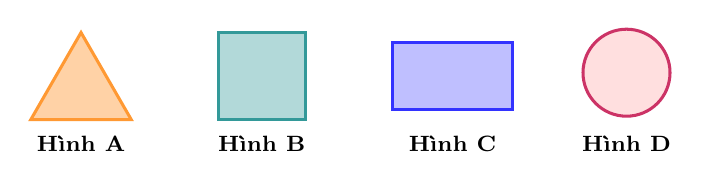
\begin{tikzpicture}[scale=0.85, baseline=(current bounding box.center)]
  \begin{scope}[shift={(0,0)}]
    \draw[fill=orange!35, draw=orange!80, line width=1.1pt] (0,0) -- (1.5,0) -- (0.75,1.3) -- cycle;
    \node[below, font=\bfseries\footnotesize] at (0.75,-0.1) {Hình A};
  \end{scope}
  \begin{scope}[shift={(2.8,0)}]
    \draw[fill=teal!30, draw=teal!80, line width=1.1pt] (0,0) rectangle (1.3,1.3);
    \node[below, font=\bfseries\footnotesize] at (0.65,-0.1) {Hình B};
  \end{scope}
  \begin{scope}[shift={(5.4,0)}]
    \draw[fill=blue!25, draw=blue!80, line width=1.1pt] (0,0.15) rectangle (1.8,1.15);
    \node[below, font=\bfseries\footnotesize] at (0.9,-0.1) {Hình C};
  \end{scope}
  \begin{scope}[shift={(8.2,0)}]
    \draw[fill=pink!50, draw=purple!80, line width=1.1pt] (0.7,0.7) circle (0.65cm);
    \node[below, font=\bfseries\footnotesize] at (0.7,-0.1) {Hình D};
  \end{scope}
\end{tikzpicture}
\end{center}
\choice
{Hình A (Hình tam giác)}
{Hình C (Hình chữ nhật)}
{Hình D (Hình tròn)}
{\True Hình B (Hình vuông)}
\loigiai{
Hình B có $4$ cạnh thẳng bằng nhau là hình vuông.\\
\textbf{Đáp án của câu hỏi là D}
}
\end{ex}

% --- CÂU 7 ---
\begin{ex} %[1D5V20]
Thực hiện tính giá trị biểu thức sau: $3 + 4 + 3 = ?$
\begin{center}

\begin{tikzpicture}[scale=0.85, baseline=(current bounding box.center)]
  \draw[fill=yellow!15, draw=orange!70, rounded corners=5pt, line width=1.1pt] (0,0) rectangle (6.5,1.2);
  \node[font=\bfseries\Large, text=orange!90!black] at (3.25,0.6) {$3 + 4 + 3 = ?$};
\end{tikzpicture}
\end{center}
\choice
{$9$}
{$8$}
{\True $10$}
{$7$}
\loigiai{
Tính: $3 + 4 = 7$, sau đó $7 + 3 = 10$.\\
\textbf{Đáp án của câu hỏi là C}
}
\end{ex}

% --- CÂU 8 ---
\begin{ex} %[1D5V20]
Tính giá trị của dãy tính trừ liên tiếp: $10 - 5 - 2 = ?$
\begin{center}
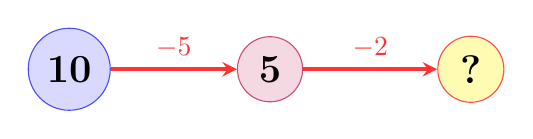
\begin{tikzpicture}[scale=0.85, baseline=(current bounding box.center)]
  \node[circle, draw=blue!70, fill=blue!15, font=\bfseries\Large, inner sep=4pt] (A) at (0,0) {10};
  \node[circle, draw=purple!70, fill=purple!15, font=\bfseries\Large, inner sep=4pt] (B) at (3,0) {5};
  \node[circle, draw=red!70, fill=yellow!30, font=\bfseries\Large, inner sep=4pt] (C) at (6,0) {?};
  \draw[->, >=stealth, line width=1.3pt, red!80] (A) -- node[above, font=\bfseries] {$- 5$} (B);
  \draw[->, >=stealth, line width=1.3pt, red!80] (B) -- node[above, font=\bfseries] {$- 2$} (C);
\end{tikzpicture}
\end{center}
\choice
{\True $3$}
{$2$}
{$4$}
{$5$}
\loigiai{
Tính: $10 - 5 = 5$, tiếp tục $5 - 2 = 3$.\\
\textbf{Đáp án của câu hỏi là A}
}
\end{ex}

\newpage

% --- CÂU 9 ---
\begin{ex} %[1D5V20]
Hộp quà bí mật chứa mấy quả bóng để khi gộp thêm $3$ quả bóng thì có tất cả $10$ quả bóng?
\begin{center}
\begin{tikzpicture}[scale=0.85, baseline=(current bounding box.center)]
  \draw[fill=yellow!30, draw=orange!80, line width=1.1pt, rounded corners=3pt] (0,0) rectangle (1.8,1.4);
  \node[font=\bfseries\Large, text=red!85!black] at (0.9,0.7) {?};
  \node[below, font=\footnotesize] at (0.9,0) {Hộp quà};
  \node[font=\bfseries\LARGE] at (2.4,0.7) {$+$};
  \draw[fill=blue!10, draw=blue!60, rounded corners=3pt] (3.0,0.2) rectangle (5.0,1.2);
  \node[font=\bfseries] at (4.0,0.7) {3 quả};
  \node[font=\bfseries\LARGE] at (5.6,0.7) {$=$};
  \draw[fill=green!10, draw=green!60!black, rounded corners=3pt] (6.2,0.2) rectangle (8.2,1.2);
  \node[font=\bfseries] at (7.2,0.7) {10 quả};
\end{tikzpicture}
\end{center}
\choice
{$6$}
{$8$}
{$5$}
{\True $7$}
\loigiai{
Ta có $7 + 3 = 10$, nên số trong hộp quà là $7$.\\
\textbf{Đáp án của câu hỏi là D}
}
\end{ex}

% --- CÂU 10 ---
\begin{ex} %[1D5V20]
Bốn chú gà con đeo thẻ các số $8, 2, 10, 5$. Sắp xếp các số theo thứ tự từ \textbf{bé đến lớn} là:
\begin{center}
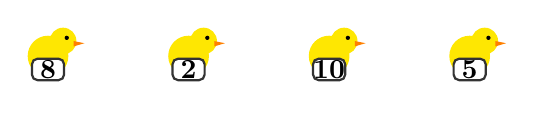
\begin{tikzpicture}[scale=0.85, baseline=(current bounding box.center)]
  \VeGaCon{0.5}{0}{8}
  \VeGaCon{2.6}{0}{2}
  \VeGaCon{4.7}{0}{10}
  \VeGaCon{6.8}{0}{5}
\end{tikzpicture}
\end{center}
\choice
{\True $2, 5, 8, 10$}
{$10, 8, 5, 2$}
{$2, 8, 5, 10$}
{$5, 2, 8, 10$}
\loigiai{
So sánh các số: $2 < 5 < 8 < 10$. Thứ tự từ bé đến lớn là $2, 5, 8, 10$.\\
\textbf{Đáp án của câu hỏi là A}
}
\end{ex}

% --- CÂU 11 ---
\begin{ex} %[1H5V20]
Ngọn tháp dưới đây được tạo thành từ bao nhiêu khối hộp chữ nhật?
\begin{center}
\begin{tikzpicture}[scale=0.85, baseline=(current bounding box.center)]
  \VeKhoiHopChuNhat[teal!45]{0}{0}{3.2}{1.0}{1.2}
  \VeKhoiHopChuNhat[teal!45]{0.6}{1.15}{2.0}{1.0}{1.2}
  \VeKhoiLapPhuong[yellow!70]{1.1}{2.3}{1.0}
  \node[right, font=\footnotesize\itshape, text=teal!80!black] at (3.8,0.6) {(Tầng 1: khối hộp)};
  \node[right, font=\footnotesize\itshape, text=teal!80!black] at (3.8,1.6) {(Tầng 2: khối hộp)};
  \node[right, font=\footnotesize\itshape, text=yellow!70!black] at (3.8,2.7) {(Tầng 3: khối lập phương)};
\end{tikzpicture}
\end{center}
\choice
{$1$ khối}
{$3$ khối}
{\True $2$ khối hộp chữ nhật}
{$4$ khối}
\loigiai{
Ngọn tháp gồm $2$ khối hộp chữ nhật ở tầng dưới và $1$ khối lập phương ở đỉnh. Vậy có $2$ khối hộp chữ nhật.\\
\textbf{Đáp án của câu hỏi là C}
}
\end{ex}

% --- CÂU 12 ---
\begin{ex} %[1H5V20]
Quan sát hình vẽ: Chú mèo bông đang ở vị trí nào so với chiếc hộp quà?
\begin{center}
\begin{tikzpicture}[scale=0.85, baseline=(current bounding box.center)]
  \VeKhoiLapPhuong[cyan!40]{0}{0}{1.8}
  % Mèo con bên phải cái hộp
  \begin{scope}[shift={(3.2,0.5)}, scale=0.6]
    \fill[orange!85] (0,0) ellipse (0.45cm and 0.35cm);
    \fill[orange!85] (0,0.5) circle (0.3cm);
    \fill[orange!85] (-0.2,0.7) -- (-0.35,1.0) -- (-0.05,0.8) -- cycle;
    \fill[orange!85] (0.2,0.7) -- (0.35,1.0) -- (0.05,0.8) -- cycle;
    \fill[black] (-0.1,0.55) circle (0.04cm);
    \fill[black] (0.1,0.55) circle (0.04cm);
    \node[below, font=\bfseries\footnotesize, text=orange!90!black] at (0,-0.4) {Mèo con};
  \end{scope}
  \node[below, font=\bfseries\footnotesize, text=blue!80!black] at (1.0,-0.2) {Hộp quà};
\end{tikzpicture}
\end{center}
\choice
{Ở bên trái hộp quà}
{\True Ở bên phải hộp quà}
{Ở trong hộp quà}
{Ở dưới gầm hộp quà}
\loigiai{
Chú mèo con đang đứng ở phía bên phải chiếc hộp quà.\\
\textbf{Đáp án của câu hỏi là B}
}
\end{ex}

\newpage

% =========================================================================
% PHẦN 2: CÂU ĐÚNG / SAI (2 CÂU, MỖI CÂU 4 Ý)
% =========================================================================
\textbf{Phần 2. Câu trắc nghiệm đúng sai}
\setcounterpageref{ex}{0}

% --- CÂU 13 ---
\begin{ex} %[1D5H20]
Trong giờ giải lao, cô giáo chia đồ chơi cho ba nhóm học sinh:
\begin{center}
\begin{tikzpicture}[scale=0.8, baseline=(current bounding box.center)]
  % Nhóm 1
  \draw[fill=pink!20, draw=purple!70, rounded corners=4pt, line width=1pt] (0,0) rectangle (3.3,1.6);
  \node[font=\bfseries\footnotesize, text=purple!90!black] at (1.65,1.25) {Nhóm 1: 5 bạn};
  \node[font=\large, text=red!80] at (1.65,0.55) {$\smiley\,\smiley\,\smiley\,\smiley\,\smiley$};
  
  % Nhóm 2
  \draw[fill=orange!15, draw=orange!70, rounded corners=4pt, line width=1pt] (4.0,0) rectangle (7.3,1.6);
  \node[font=\bfseries\footnotesize, text=orange!90!black] at (5.65,1.25) {Nhóm 2: 3 bạn};
  \node[font=\large, text=orange!90] at (5.65,0.55) {$\smiley\,\smiley\,\smiley$};
  
  % Nhóm 3
  \draw[fill=green!15, draw=green!70!black, rounded corners=4pt, line width=1pt] (8.0,0) rectangle (11.3,1.6);
  \node[font=\bfseries\footnotesize, text=green!80!black] at (9.65,1.25) {Nhóm 3: 2 bạn};
  \node[font=\large, text=green!80!black] at (9.65,0.55) {$\smiley\,\smiley$};
\end{tikzpicture}
\end{center}
Xét tính Đúng hay Sai của các khẳng định sau:
\choiceTF
{\True Tổng số học sinh của cả ba nhóm là $5 + 3 + 2 = 10$ bạn}
{Nhóm 1 có ít học sinh hơn Nhóm 2}
{\True Nhóm 1 nhiều hơn Nhóm 3 là $5 - 2 = 3$ bạn}
{Nếu gộp Nhóm 2 và Nhóm 3 thì được số bạn nhiều hơn Nhóm 1}
\loigiai{
Số học sinh: Nhóm 1: 5 bạn; Nhóm 2: 3 bạn; Nhóm 3: 2 bạn.\\
a) Tổng số bạn: $5 + 3 + 2 = 10$ bạn $\to$ \textbf{Đúng}.\\
b) Nhóm 1 có 5 bạn nhiều hơn Nhóm 2 (3 bạn) $\to$ \textbf{Sai}.\\
c) Hiệu giữa Nhóm 1 và Nhóm 3: $5 - 2 = 3$ bạn $\to$ \textbf{Đúng}.\\
d) Gộp Nhóm 2 và 3 được $3 + 2 = 5$ bạn, bằng Nhóm 1 chứ không nhiều hơn $\to$ \textbf{Sai}.
}
\end{ex}

% --- CÂU 14 ---
\begin{ex} %[1H5V20]
Bạn Bình dùng các khối gỗ để ghép thành một lâu đài đồ chơi:
\begin{center}
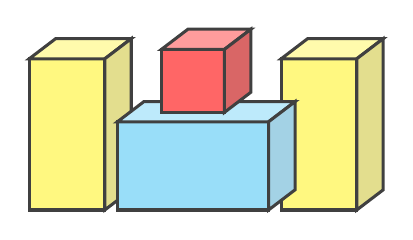
\begin{tikzpicture}[scale=0.8, baseline=(current bounding box.center)]
  % Hai tháp 2 bên
  \VeKhoiHopChuNhat[yellow!50]{0}{0}{1.2}{2.4}{1.0}
  \VeKhoiHopChuNhat[yellow!50]{4.0}{0}{1.2}{2.4}{1.0}
  % Tường thành ở giữa
  \VeKhoiHopChuNhat[cyan!40]{1.4}{0}{2.4}{1.4}{1.0}
  % Khối lập phương trên đỉnh tường
  \VeKhoiLapPhuong[red!60]{2.1}{1.55}{1.0}
\end{tikzpicture}
\end{center}
Xét tính Đúng hay Sai của các khẳng định sau:
\choiceTF
{\True Lâu đài có $3$ khối hộp chữ nhật}
{Khối trên đỉnh tường thành là khối hộp chữ nhật}
{\True Khối lập phương ở vị trí cao hơn tường thành}
{Lâu đài có tất cả $6$ khối lập phương}
\loigiai{
a) Hai tháp và một tường thành là $3$ khối hộp chữ nhật $\to$ \textbf{Đúng}.\\
b) Khối trên đỉnh là khối lập phương (màu đỏ) $\to$ \textbf{Sai}.\\
c) Khối lập phương nằm trên đỉnh nên ở vị trí cao hơn $\to$ \textbf{Đúng}.\\
d) Lâu đài chỉ có $1$ khối lập phương (không phải 6) $\to$ \textbf{Sai}.
}
\end{ex}

\newpage

% =========================================================================
% PHẦN 3: CÂU TRẢ LỜI NGẮN (6 CÂU)
% =========================================================================
\textbf{Phần 3. Câu trắc nghiệm trả lời ngắn}
\setcounterpageref{ex}{0}

% --- CÂU 15 ---
\begin{ex} %[1D5H20]
Điền số thích hợp vào ô trống trên tia số dưới đây:
\begin{center}
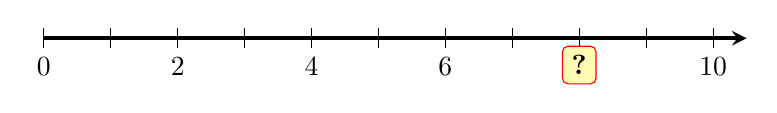
\begin{tikzpicture}[scale=0.85, baseline=(current bounding box.center)]
  \draw[->, >=stealth, line width=1.3pt] (0,0) -- (10.5,0);
  \foreach \x in {0,...,10}{
    \draw (\x,0.15) -- (\x,-0.15);
  }
  \node[below] at (0,-0.15) {0}; \node[below] at (2,-0.15) {2}; \node[below] at (4,-0.15) {4};
  \node[below] at (6,-0.15) {6};
  \node[draw=red, fill=yellow!30, rounded corners=2pt, font=\bfseries] at (8,-0.4) {?};
  \node[below] at (10,-0.15) {10};
\end{tikzpicture}
\end{center}
\textbf{Trả lời:} \raisebox{-2pt}{\framebox[1.5cm]{\phantom{1}}}
\loigiai{
Quy luật dãy số chẵn: $0, 2, 4, 6, \mathbf{8}, 10$. Số cần điền là $8$.\\
\textbf{Đáp số:} 8
}
\end{ex}

% --- CÂU 16 ---
\begin{ex} %[1D5H20]
Tính kết quả của phép tính: $10 - 6 + 4 = ?$
\begin{center}
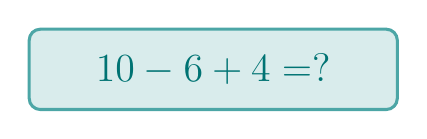
\begin{tikzpicture}[scale=0.85, baseline=(current bounding box.center)]
  \draw[fill=teal!15, draw=teal!70, rounded corners=4pt, line width=1.1pt] (0,0) rectangle (5.5,1.2);
  \node[font=\bfseries\Large, text=teal!90!black] at (2.75,0.6) {$10 - 6 + 4 = ?$};
\end{tikzpicture}
\end{center}
\textbf{Trả lời:} \raisebox{-2pt}{\framebox[1.5cm]{\phantom{1}}}
\loigiai{
Tính: $10 - 6 = 4$, sau đó $4 + 4 = 8$.\\
\textbf{Đáp số:} 8
}
\end{ex}

% --- CÂU 17 ---
\begin{ex} %[1H5V20]
Hình con cá dưới đây được ghép bởi bao nhiêu hình tam giác?
\begin{center}
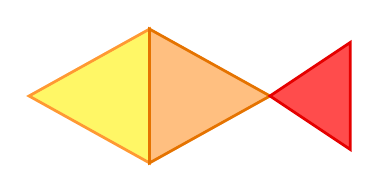
\begin{tikzpicture}[scale=0.85, baseline=(current bounding box.center)]
  % Thân cá ghép từ 2 tam giác
  \draw[fill=yellow!60, draw=orange!80, line width=1pt] (0,0) -- (1.8,1.0) -- (1.8,-1.0) -- cycle;
  \draw[fill=orange!50, draw=orange!90!black, line width=1pt] (1.8,1.0) -- (3.6,0) -- (1.8,-1.0) -- cycle;
  % Đuôi cá là 1 tam giác
  \draw[fill=red!70, draw=red!90!black, line width=1pt] (3.6,0) -- (4.8,0.8) -- (4.8,-0.8) -- cycle;
\end{tikzpicture}
\end{center}
\textbf{Trả lời:} \raisebox{-2pt}{\framebox[1.5cm]{\phantom{1}}}
\loigiai{
Thân cá có $2$ hình tam giác, đuôi cá có $1$ hình tam giác. Tổng cộng có: $2 + 1 = 3$ hình tam giác.\\
\textbf{Đáp số:} 3
}
\end{ex}

% --- CÂU 18 ---
\begin{ex} %[1D5V20]
Bến xe có $8$ chiếc xe buýt, sau đó có $3$ chiếc xe buýt xuất bến chở khách đi. Hỏi bến xe còn lại bao nhiêu chiếc xe buýt?
\begin{center}
\begin{tikzpicture}[scale=0.85, baseline=(current bounding box.center)]
  \draw[fill=gray!15, draw=black!60, rounded corners=6pt] (0,0) rectangle (7.5,1.6);
  \node[font=\bfseries\footnotesize, text=blue!90!black] at (3.75,1.25) {Bến xe: 8 xe ban đầu -- Rời bến: 3 xe};
  \node[font=\bfseries\Large, text=red!80!black] at (3.75,0.55) {$8 - 3 = ?\text{ xe}$};
\end{tikzpicture}
\end{center}
\textbf{Trả lời:} \raisebox{-2pt}{\framebox[1.5cm]{\phantom{1}}}
\loigiai{
Số xe còn lại là: $8 - 3 = 5$ (xe buýt).\\
\textbf{Đáp số:} 5
}
\end{ex}

% --- CÂU 19 ---
\begin{ex} %[1D5V20]
Tìm số thích hợp điền vào đỉnh tháp số cộng dưới đây (số ở ô trên bằng tổng hai số ở hai ô kề nhau bên dưới):
\begin{center}
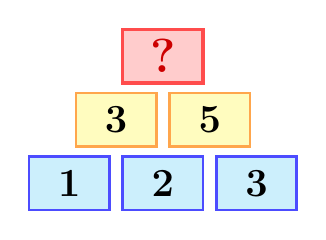
\begin{tikzpicture}[scale=0.85, baseline=(current bounding box.center)]
  % Tầng 1
  \draw[fill=cyan!20, draw=blue!70, line width=1pt] (0,0) rectangle (1.2,0.8); \node[font=\bfseries\Large] at (0.6,0.4) {1};
  \draw[fill=cyan!20, draw=blue!70, line width=1pt] (1.4,0) rectangle (2.6,0.8); \node[font=\bfseries\Large] at (2.0,0.4) {2};
  \draw[fill=cyan!20, draw=blue!70, line width=1pt] (2.8,0) rectangle (4.0,0.8); \node[font=\bfseries\Large] at (3.4,0.4) {3};
  % Tầng 2
  \draw[fill=yellow!25, draw=orange!70, line width=1pt] (0.7,0.95) rectangle (1.9,1.75); \node[font=\bfseries\Large] at (1.3,1.35) {3};
  \draw[fill=yellow!25, draw=orange!70, line width=1pt] (2.1,0.95) rectangle (3.3,1.75); \node[font=\bfseries\Large] at (2.7,1.35) {5};
  % Tầng 3
  \draw[fill=red!20, draw=red!70, line width=1.2pt] (1.4,1.9) rectangle (2.6,2.7);
  \node[font=\bfseries\LARGE, text=red!80!black] at (2.0,2.3) {?};
\end{tikzpicture}
\end{center}
\textbf{Trả lời:} \raisebox{-2pt}{\framebox[1.5cm]{\phantom{1}}}
\loigiai{
Ô ở đỉnh là tổng của $3$ và $5$: $3 + 5 = 8$.\\
\textbf{Đáp số:} 8
}
\end{ex}

% --- CÂU 20 ---
\begin{ex} %[1H5V20]
Có bao nhiêu khối lập phương màu vàng trong hình xếp dưới đây?
\begin{center}
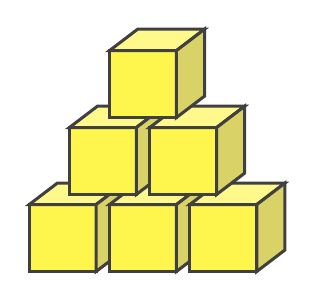
\begin{tikzpicture}[scale=0.85, baseline=(current bounding box.center)]
  \VeKhoiLapPhuong[yellow!70]{0}{0}{1.0}
  \VeKhoiLapPhuong[yellow!70]{1.2}{0}{1.0}
  \VeKhoiLapPhuong[yellow!70]{2.4}{0}{1.0}
  \VeKhoiLapPhuong[yellow!70]{0.6}{1.15}{1.0}
  \VeKhoiLapPhuong[yellow!70]{1.8}{1.15}{1.0}
  \VeKhoiLapPhuong[yellow!70]{1.2}{2.3}{1.0}
\end{tikzpicture}
\end{center}
\textbf{Trả lời:} \raisebox{-2pt}{\framebox[1.5cm]{\phantom{1}}}
\loigiai{
Đếm theo tầng: $3 + 2 + 1 = 6$ khối lập phương.\\
\textbf{Đáp số:} 6
}
\end{ex}
